% Author: Maxwell Chen, Taejin Hwang
% Email: maxhchen@berkeley.edu, taejin@berkeley.edu

\qns{Filter Design}

\meta{
For mentors, this problem is really long and it's okay to not get to finish this question or even get to it.
If there's not enough time, just graph the graphs for the students.
}

Suppose you have been hired to design a biomedical sensor that can detect and output recordings of Alpha brainwaves in the frequency range $8 \, \text{Hz}$ to $12 \, \text{Hz}$.
Unfortunately, our sensor is faulty: it is also picking up Gamma brainwaves in the frequency range $40 \, \text{Hz}$ to $100 \, \text{Hz}$, interfering with our ability to get clean recordings of alpha brainwaves.
We want to create a new design for our sensor that can remove this interference, giving us a clearer signal.

For the following, it's recommended that you graph the plots with a computer.

\begin{enumerate}
  \qitem What kind of filter could you use to remove this interference?

  \ws{
  \vspace{75px}
  }

  \sol {
  We should use a low-pass filter. The interference is at a higher frequency than our desired signal, so we filter out the higher frequencies and keep the lower frequencies.
  }


  \qitem Assume we only have access to resistors and capacitors. \textbf{Sketch the corresponding filter circuit and write out its transfer function.}

  \ws{
  \vspace{150px}
  }

  \sol {
  $$H(j \omega) = \frac{\widetilde{Z}_{out}}{\widetilde{Z}_{in}} = \frac{\frac{1}{j\omega C}}{R + \frac{1}{j \omega C}} = \frac{1}{1 + j\omega RC} = \frac{1}{1 + j \frac{\omega}{\omega_{c}}}$$.

  \begin{center}
  \begin{circuitikz} \draw
    (0, 0) node[ground] {}
      to [sV, l_=$V_{in}$] (0, 4)
      to [R = R] (4, 4)
      to [C = C] (4, 0)
      node[ground] {}

    (4, 3) to[short, -o] (6, 3) node[anchor=west] (A) {A}

    (4, 1) to[short, -o] (6, 1) node[anchor=west] (B) {B}

    (A) to[open, l^=$V_{out}$] (B)
  ;\end{circuitikz}
\end{center}

  }

  \qitem $\omega_{c} = \frac{1}{RC}$ is the cutoff frequency which determines the frequency at which our filter starts attenuating the signal. \textbf{Should we maximize or minimize $\omega_{c}$ to remove as much of the interference as possible?}

  \ws{
  \vspace{75px}
  }

  \sol {
  We should minimize the cutoff frequency. The transfer function will start filtering frequencies sooner, meaning that we maximize the amount by which higher frequencies are attenuated.
  }

  \qitem Say we can set our cutoff frequency to $10 \, \text{Hz}$, $20 \, \text{Hz}$, $32 \, \text{Hz}$, $100 \, \text{Hz}$, or $120 \, \text{Hz}$. Which is the best cutoff frequency, and why?

  \ws{
  \vspace{75px}
  }

  \sol {
  20Hz. This is the lowest cutoff frequency we can choose; the Gamma brainwaves will be attenuated more if we choose 20Hz than 32Hz because the transfer function will start filtering at a lower frequency. 10Hz is too low and risks cutting off Alpha brainwaves.
  }

  \qitem We only have a 3.3 k$\Omega$ resistor in our workstation. What capacitor value should we use for our filter?

  \ws{
  \vspace{75px}
  }

  \sol {
  If we want a cutoff frquency of 20Hz, then $f = \frac{\omega_{c}}{2 \pi} = \frac{1}{2 \pi RC} = 20Hz$. So, $C = \frac{1}{2 \pi \cdot 33 \cdot 10^{3} \Omega \cdot 20Hz} = 2.41 \, \mu$F.
  }

  \qitem Use a computer to plot the magnitude and phase response of this filter.

  \ws{
  \vspace{200px}
  }

  \sol {
  \newpage
  \begin{figure}[h]
  \centering

  \textbf{Magnitude plot:}

  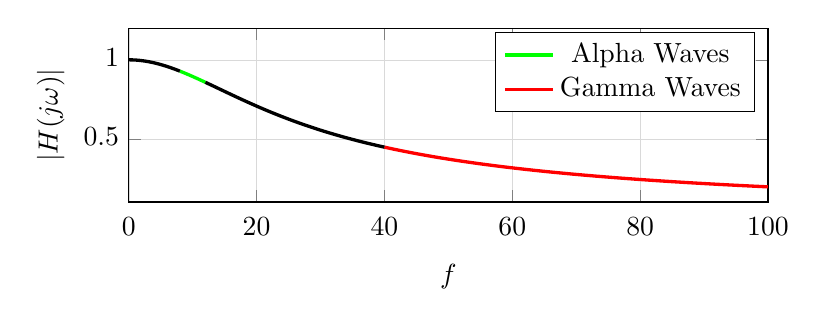
\begin{tikzpicture}[
    declare function={
      mag(\omega)= 1 / sqrt(1 + (\omega * 2 * pi * 3300 * 2.41*10^(-6))^2);
      alpha(\omega) = mag(\omega) * (\omega >=8) * (\omega <= 12);
      gamma(\omega) = mag(\omega) * (\omega > 40);
      mid1(\omega) = mag(\omega) * (\omega >= 0) * (\omega <= 8);
      mid2(\omega) = mag(\omega) * (\omega >= 12) * (\omega <= 40);
      % Straight line bode approximation
      % mag(\omega)= (\omega < 10^8) * (1) +
      %           (\omega >= 10^8) * (10^8 / \omega)
    }
  ]
  \begin{axis}[
    typeset ticklabels with strut,
    ymin=0.1, ymax=1.2, ylabel=$|H(j \omega)|$,
    xmin=0.0001, xmax=100, xlabel=$f$,
    % xticklabels={$0.02$,$0.2$,$2$,$20$,$200$, $2000$, $20000$},
    domain=0.0001:100,
    grid=both, grid style={line width=.1pt, draw=gray!30},
    width=\textwidth * 0.8,
    height=\textwidth / 3.2,
  ]
    \addplot [domain=8.001:11.999,green,very thick,samples = 200] {alpha(x)};
    \addlegendentry{Alpha Waves}
    \addplot [domain=40.001:100,red,very thick,samples = 200] {gamma(x)};
    \addlegendentry{Gamma Waves}
    \addplot [domain=0.001:7.999, black,very thick,samples = 200] {mid1(x)};
    \addplot [domain=12.001:39.999,black,very thick,samples = 200] {mid2(x)};
    \end{axis}
  \end{tikzpicture}
  \end{figure}

  \begin{figure}[h]
  \centering

  \textbf{Phase plot:}

  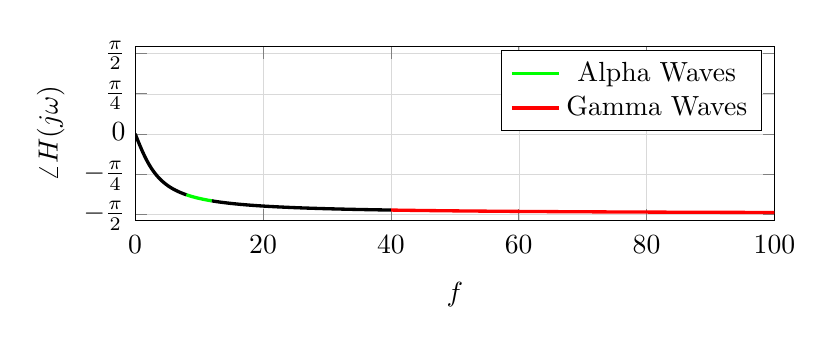
\begin{tikzpicture}[
    declare function={
      phase(\omega)= -rad(atan(2 * pi * \omega / (20)));
      alpha(\omega) = phase(\omega) * (\omega >=8) * (\omega <= 12);
      gamma(\omega) = phase(\omega) * (\omega > 40);
      mid1(\omega) = phase(\omega) * (\omega >= 0) * (\omega <= 8);
      mid2(\omega) = phase(\omega) * (\omega >= 12) * (\omega <= 40);
      % Straight line bode approximation
      % mag(\omega)= (\omega < 10^8) * (1) +
      %           (\omega >= 10^8) * (10^8 / \omega)
    }
  ]
  \begin{axis}[
    typeset ticklabels with strut,
    ymin= -1.7, ymax=1.7, ylabel=$\angle H(j \omega)$, ytick={-pi/2, -pi/4, 0, pi/4, pi/2},
    yticklabels={$-\frac{\pi}{2}$,$-\frac{\pi}{4}$,$0$,$\frac{\pi}{4}$,$\frac{\pi}{2}$},
    xmin=0.0001, xmax=100, xlabel=$f$,
    % xticklabels={$0.02$,$0.2$,$2$,$20$,$200$, $2000$, $20000$},
    domain=0.0001:1000,
    grid=both, grid style={line width=.1pt, draw=gray!30},
    width=\textwidth * 0.8,
    height=\textwidth / 3.2,
  ]
    \addplot [domain=8.001:11.999,green,very thick,samples = 200] {alpha(x)};
    \addlegendentry{Alpha Waves}
    \addplot [domain=40.001:100,red,very thick,samples = 200] {gamma(x)};
    \addlegendentry{Gamma Waves}
    \addplot [domain=0.001:7.999, black,very thick,samples = 200] {mid1(x)};
    \addplot [domain=12.001:39.999,black,very thick,samples = 200] {mid2(x)};
    \end{axis}
  \end{tikzpicture}
  \end{figure}
  }

  \qitem We can look at the magnitude phase plots of the previous part, realize that the performance our filter is rather poor.
  $|H(j \omega)|$ at $\SI{40}{\hertz}$ is still around $0.5.$ This is because the Alpha and Delta brainwaves are very close together in frequency, and it takes an entire magnitude for the magnitude of the transfer function to drop by a factor of $10.$ \vskip 1pt
  To combat this, we can cascade two of the low pass filters from the previous part with the same resistor and capacitor values, with a buffer in between as shown below:

  \begin{center}
  \begin{circuitikz}[scale = 0.8, transform shape] \draw
    (0, 2) node[ground] (lground) {}
      to [sV, l_=$v_{in}$] (0, 4)
      to [R = $R$] (4, 4)
      to [C = $C$] (4, 2)
      node[ground] (mground) {}

    (7, 3.5) node[op amp, yscale=-1] (opamp) {}
      (opamp.+) to [short] (4, 4)
      (opamp.-) -| (5.5, 2)
      (opamp.out) |- (5.5, 2)
      (opamp.out) to [R = $R$] (12, 3.5)
      to [C = $C$] (12, 0.5)
      node[ground] (rground) {}

    (12, 3.5) to[short, -o] (14, 3.5) node[anchor=west] (A) {A}

    (12, 1) to[short, -o] (14, 1) node[anchor=west] (B) {B}

    (A) to[open, l^=$v_{out}$] (B)
  ;\end{circuitikz}
\end{center}


  What is the transfer function $H(j \omega),$ and see what the response looks like on a computer. In addition, what would happen if we cascaded a large number of filters together?

  \ws{
  \vspace{200px}
  }

  \sol {
  The transfer function of this circuit would be the product of two low-pass transfer functions. \vskip 1pt

  \begin{equation}
  H(j \omega) = \frac{1}{1 + j \omega RC} \cdot \frac{1}{1 + j \omega RC}
  \end{equation}

  This will also have low-pass behavior, and will have a faster rate of cutoff after the cutoff frequency. \vskip 1pt
  However, notice that as $n$ gets larger, $|H(j \omega)|$ drops off, and we may have to use an amplifier to restore the gain:

  \begin{figure}[h]
  \centering

  \textbf{Magnitude Plot (One Buffer):}

  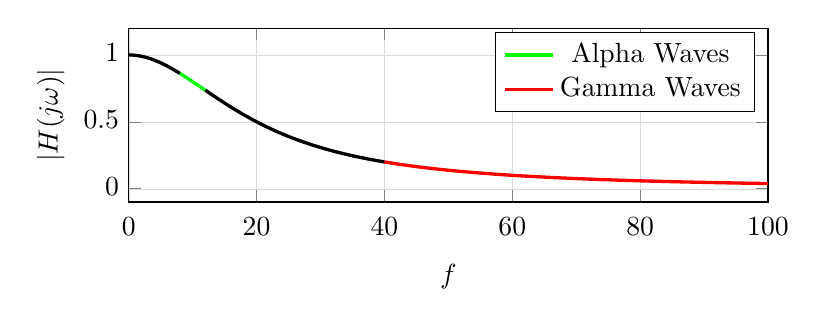
\begin{tikzpicture}[
    declare function={
      mag(\omega)= 1 / sqrt(1 + (\omega * 2 * pi * 3300 * 2.41*10^(-6))^2)^(2);
      alpha(\omega) = mag(\omega) * (\omega >=8) * (\omega <= 12);
      gamma(\omega) = mag(\omega) * (\omega > 40);
      mid1(\omega) = mag(\omega) * (\omega >= 0) * (\omega <= 8);
      mid2(\omega) = mag(\omega) * (\omega >= 12) * (\omega <= 40);
      % Straight line bode approximation
      % mag(\omega)= (\omega < 10^8) * (1) +
      %           (\omega >= 10^8) * (10^8 / \omega)
    }
  ]
  \begin{axis}[
    typeset ticklabels with strut,
    ymin=-0.1, ymax=1.2, ylabel=$|H(j \omega)|$,
    xmin=0.0001, xmax=100, xlabel=$f$,
    domain=0.0001:100,
    grid=both, grid style={line width=.1pt, draw=gray!30},
    width=\textwidth * 0.8,
    height=\textwidth / 3.2,
  ]
    \addplot [domain=8.001:11.999,green,very thick,samples = 200] {alpha(x)};
    \addlegendentry{Alpha Waves}
    \addplot [domain=40.001:100,red,very thick,samples = 200] {gamma(x)};
    \addlegendentry{Gamma Waves}
    \addplot [domain=0.001:7.999, black,very thick,samples = 200] {mid1(x)};
    \addplot [domain=12.001:39.999,black,very thick,samples = 200] {mid2(x)};
    \end{axis}
  \end{tikzpicture}
  \end{figure}

  In fact we can cascade, a series of filters, to get an even better rate of dropoff. The plots for $5$ and $10$ cascaded filters are shown below.

  \begin{figure}[h]
  \centering

  \textbf{Magnitude Plot (Five Buffers):}

  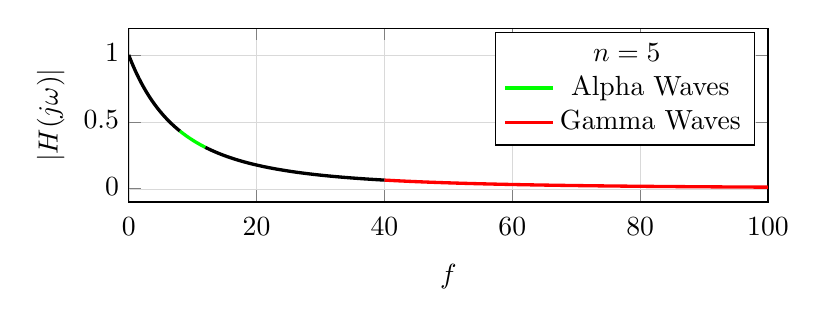
\begin{tikzpicture}[
    declare function={
      mag(\omega)= 1 / sqrt(1 + (\omega * 2 * pi * 3300 * 2.41*10^(-6)))^(5);
      alpha(\omega) = mag(\omega) * (\omega >=8) * (\omega <= 12);
      gamma(\omega) = mag(\omega) * (\omega > 40);
      mid1(\omega) = mag(\omega) * (\omega >= 0) * (\omega <= 8);
      mid2(\omega) = mag(\omega) * (\omega >= 12) * (\omega <= 40);
      % Straight line bode approximation
      % mag(\omega)= (\omega < 10^8) * (1) +
      %           (\omega >= 10^8) * (10^8 / \omega)
    }
  ]
  \begin{axis}[
    typeset ticklabels with strut,
    ymin=-0.1, ymax=1.2, ylabel=$|H(j \omega)|$,
    xmin=0.0001, xmax=100, xlabel=$f$,
    domain=0.0001:100,
    grid=both, grid style={line width=.1pt, draw=gray!30},
    width=\textwidth * 0.8,
    height=\textwidth / 3.2,
  ]
    \addlegendimage{empty legend};
    \addlegendentry{\hspace{-.6cm}$n = 5$};
    \addplot [domain=8.001:11.999,green,very thick,samples = 200] {alpha(x)};
    \addlegendentry{Alpha Waves}
    \addplot [domain=40.001:100,red,very thick,samples = 200] {gamma(x)};
    \addlegendentry{Gamma Waves}
    \addplot [domain=0.001:7.999, black,very thick,samples = 200] {mid1(x)};
    \addplot [domain=12.001:39.999,black,very thick,samples = 200] {mid2(x)};
    \end{axis}
  \end{tikzpicture}
  \end{figure}

  \begin{figure}[h]
  \centering

  \textbf{Magnitude Plot (Ten Buffers):}

  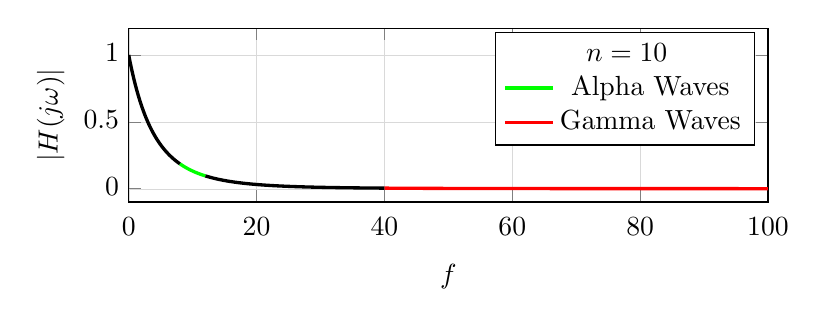
\begin{tikzpicture}[
    declare function={
      mag(\omega)= 1 / sqrt(1 + (\omega * 2 * pi * 3300 * 2.41*10^(-6)))^(10);
      alpha(\omega) = mag(\omega) * (\omega >=8) * (\omega <= 12);
      gamma(\omega) = mag(\omega) * (\omega > 40);
      mid1(\omega) = mag(\omega) * (\omega >= 0) * (\omega <= 8);
      mid2(\omega) = mag(\omega) * (\omega >= 12) * (\omega <= 40);
      % Straight line bode approximation
      % mag(\omega)= (\omega < 10^8) * (1) +
      %           (\omega >= 10^8) * (10^8 / \omega)
    }
  ]
  \begin{axis}[
    typeset ticklabels with strut,
    ymin=-0.1, ymax=1.2, ylabel=$|H(j \omega)|$,
    xmin=0.0001, xmax=100, xlabel=$f$,
    domain=0.0001:100,
    grid=both, grid style={line width=.1pt, draw=gray!30},
    width=\textwidth * 0.8,
    height=\textwidth / 3.2,
  ]
    \addlegendimage{empty legend};
    \addlegendentry{\hspace{-.6cm}$n = 10$};
    \addplot [domain=8.001:11.999,green,very thick,samples = 200] {alpha(x)};
    \addlegendentry{Alpha Waves}
    \addplot [domain=40.001:100,red,very thick,samples = 200] {gamma(x)};
    \addlegendentry{Gamma Waves}
    \addplot [domain=0.001:7.999, black,very thick,samples = 200] {mid1(x)};
    \addplot [domain=12.001:39.999,black,very thick,samples = 200] {mid2(x)};
    \end{axis}
  \end{tikzpicture}
  \end{figure}

  }

  \qitem Now, let's say that our filter is successful at removing the interference we initially detected. We now notice that there is another source of interference--Delta brainwaves--in the frequency range 0.5Hz to 4Hz. \textbf{How could we modify our design to remove both sources of interference and get a clear recording of Alpha brainwaves?} Suppose you do not have access to an op-amp, but you do have access to an inductor.

  \ws{
  \vspace{200px}
  }

  \sol {
  Replace our low-pass filter with a bandpass filter. This will attenuate both sources of noise and leave our frequency band for Alpha brainwaves intact for our sensor to record.

  To design our bandpass, we can use the following circuit:

  \begin{center}
  \begin{circuitikz}[scale=0.8]
      \draw (0,4) 
      to [sV, l= $V_s$] (0,0)
      (0,4)
      to [C = $C$] (3,4)
      to [L = $L$,] (6,4)
      to [short] (8,4)
      to [R = $R$] (8,0)  
      to [short] (0,0)
      (8, 4) to[short, -o] (9, 4) node[anchor=west] (+) {+}
      (8, 0) to[short, -o] (9, 0) node[anchor=west] (-) {-}
      (+) to[open, l^=$\widetilde{V}_{\text{out}}$] (-)
      ;
  \end{circuitikz}
\end{center}

  Using previous phasor analysis techniques, we can see this as a voltage divider by taking the capacitor and inductor as one impedance in series.
  $$H(j \omega) = \frac{R}{R + j \omega L + \frac{1}{j \omega C}} = \frac{j \omega RC}{1 + j \omega RC + (j \omega)^{2} LC}$$
  }

  \qitem Where would you want to set the cutoff frequencies?

  \ws{
  \vspace{100px}
  }

  \sol {
    We currently want to capture Alpha brainwaves running at 8 to 12 Hz, while filtering out Gamma brainwaves at 40 to 100 Hz, and Delta brainwaves at 0.5 to 4 Hz. We want to space our cutoff frequences as far apart as possible, but also try to put the center frequency as the average of the desired frequency range. Therefore, to space away the Deltas while keeping the Alphas, the low frequency should be set to $\SI{6}{\hertz}.$ The high frequency can vary, You can pick a high cutoff of $\SI{14}{\hertz},$ to put $\SI{10}{\hertz}$ in the center, or you can also choose $\SI{26}{\hertz}$ in between $12$ and $40$ to create a much larger bandwith.
  }

  \qitem How can we calculate the cutoff frequencies for our filter in terms of R, L, and C?

  \ws{
  \vspace{200px}
  }

  \meta {
    We use $\sqrt{\frac{1}{2}}$ since it is the half power point.
  }

  \sol {
    Remember that in order to find the cutoff frequencies, we find the frequencies at which $|H(j \omega)| = \frac{1}{\sqrt{2}}.$
    $$|H(j \omega)| = \frac{\omega RC}{\sqrt{(1 - \omega^{2} LC)^2 + (\omega RC)^2}} = \frac{1}{\sqrt{2}}$$
    Squaring both sides, we get:
    $$\Big( \frac{\omega RC}{\sqrt{(1 - \omega^{2} LC)^2 + (\omega RC)^2}} \Big)^{2} = \frac{(\omega RC)^2}{(1 - \omega^{2} LC)^2 + (\omega RC)^2} = \frac{1}{2}$$
    Cross multiplying, we get:
    $$(1 - \omega^{2} LC)^2 + (\omega RC)^2 = 2 (\omega RC)^2 \ \ \text{or} \ \ (1 - \omega^{2} LC)^2 = (\omega RC)^2$$
    We take the square root of both sides, and taking the negative case into account,
    $$(1 - \omega^{2} LC) = \pm \omega RC$$
    Now, we can use the quadratic formula twice, and note that we'll have four solutions, but we will only consider the positive valued ones.
    $$\omega = \pm \frac{R}{2L} + \sqrt{\big(\frac{R}{2L}\big)^2 + \frac{1}{LC}}$$
  }

  \clearpage

  \qitem Let's pick values of $R, L,$ and $C$ to set our cutoff frequencies to those picked in part (i).
  Suppose you have a $\SI{500}{\ohm}$ resistor. What values should you pick for your capacitior and inductor?

  \ws{
  \vspace{200px}
  }

  \sol {
    From the previous part, our cutoff frequencies are:
    $$\omega_{h} = \frac{R}{2L} + \sqrt{\big(\frac{R}{2L}\big)^2 + \frac{1}{LC}}, \ \ \text{and} \ \ \omega_{l} = -\frac{R}{2L} + \sqrt{\big(\frac{R}{2L}\big)^2 + \frac{1}{LC}}.$$
    This means that our bandwith is $\Delta \omega = \omega_{h} - \omega_{l} = \frac{R}{L}.$ \vskip 1pt
    We want to design our circuit with bandwith $\omega = 2 \pi f.$
    We will pick a low cutoff frequency, $f_{l} = \SI{6}{\hertz}$ since that will give us the most bandwith possible and is equidistant from the Alpha and Delta waves. \vskip 1pt
    For the high frequency, we can pick $f_{h} = \SI{14}{\hertz},$ to put the center frequency at $\SI{10}{\hertz}.$ meaning our bandwith will be $\SI{8}{\hertz}$ or $\SI{16 \pi}{\radian\per\second}.$ \vskip 0.5pt

    Alternatively, we can pick a high cutoff of $f_{h} = \SI{26}{\hertz},$ to give a larger bandwith of $\SI{20}{\hertz}$ or $\SI{40 \pi}{\radian\per\second}.$ Therefore since $\frac{R}{L} = \ \Delta \omega, L = \frac{R}{16 \pi} = \frac{500}{16 \pi} = \SI{9.95}{\henry}.$
    Had we picked $f_{h} = \SI{26}{\hertz},$ then $\frac{R}{40 \pi}. = \frac{500}{40 \pi} = \SI{3.98}{\henry}$ \vskip 2pt
    The center frequency, is $\omega_{center} = \frac{1}{2}(\omega_{l} + \omega_{h}) = \sqrt{\big(\frac{R}{2L} \big)^2 + \frac{1}{LC}}.$ We want to design our circuit with center frequency at either $\SI{10}{\hertz} = \SI{20 \pi}{\radian\per\second}$ or $\SI{16}{\hertz}$ or $\SI{32\pi}{\radian\per\second}.$ \vskip 0.5pt

    Therefore, we can pick the value for our capacitor accordingly.
    $$\big(\frac{R}{2L} \big)^2 + \frac{1}{LC} = 400 \pi^2 \ \ \text{so} \ \ C = \frac{1}{L(400 \pi^2 - (\frac{R}{2L})^2)} = \SI{30.3}{\micro\farad}$$

    $$\big(\frac{R}{2L} \big)^2 + \frac{1}{LC} = 1024 \pi^2 \ \ \text{so} \ \ C = \frac{1}{L(1024 \pi^2 - (\frac{R}{2L})^2)} = \SI{40.8}{\micro\farad}$$
  }

  \clearpage

  \qitem Plot the frequency response of the filter designed above using the resistor, capacitor and inductor values picked in the previous part. You should plot the frequency response on a computer.

  \ws{
  \vspace{200px}
  }

  \sol {
  We can plot this on a computer by plugging in our values for $R, L, C$ into the magnitude equation:
  \begin{equation}
  |H(j \omega)| = \frac{\omega R C}{\sqrt{(1 - \omega^2 LC)^2 + (\omega RC)^2}}
  \end{equation}
  Notice that our signal is attenuated for values of $f$ between $0.5$ and $4,$ and it is also attenuated for values of $f$ above $40.$
  Lastly, for values of $f$ between $8$ and $\SI{12}{\hertz},$ the transfer function is close to $1.$ \vskip 1pt

  The plot of $|H(j \omega)|$ is below for both choices of $R,L,C:$
  \begin{figure}[h]
  \centering

  \textbf{Magnitude Plot:}

  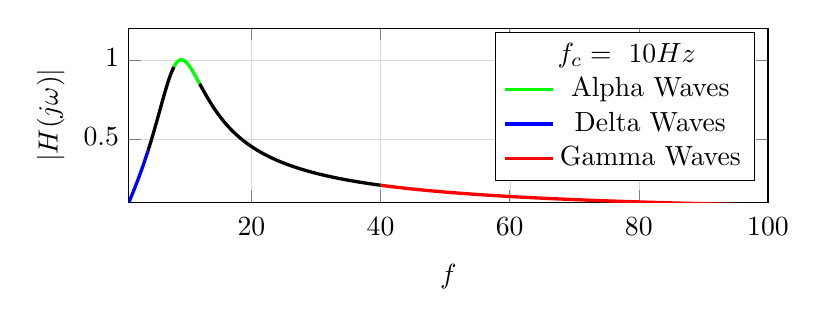
\begin{tikzpicture}[
    declare function={
      mag1(\omega)= \omega * 2 * pi * 0.015157613627799554;
      mag2(\omega)= 1 /sqrt((1 - (\omega * 2 * pi)^2 * 0.00030155114179267195)^2 + (\omega * 2 * pi * 0.015157613627799554)^2);
      mag(\omega) = mag1(\omega) * mag2(\omega);
      alpha(\omega) = mag(\omega) * (\omega >=8) * (\omega <= 12);
      delta(\omega) = mag(\omega) * (\omega <= 4);
      gamma(\omega) = mag(\omega) * (\omega > 40);
      mid1(\omega) = mag(\omega) * (\omega >= 4) * (\omega <= 8);
      mid2(\omega) = mag(\omega) * (\omega >= 12) * (\omega <= 40);
      % Straight line bode approximation
      % mag(\omega)= (\omega < 10^8) * (1) +
      %           (\omega >= 10^8) * (10^8 / \omega)
    }
  ]
  \begin{axis}[
    typeset ticklabels with strut,
    ymin=0.1, ymax=1.2, ylabel=$|H(j \omega)|$,
    xmin=1, xmax=100, xlabel=$f$,
    % xticklabels={$0.02$,$0.2$,$2$,$20$,$200$, $2000$, $20000$},
    domain=1:1000,
    grid=both, grid style={line width=.1pt, draw=gray!30},
    width=\textwidth * 0.8,
    height=\textwidth / 3.2,
  ]
    \addlegendimage{empty legend};
    \addlegendentry{\hspace{-.6cm}$f_{c} = \ 10 Hz$};
    \addplot [domain=8.001:11.999,green,very thick,samples = 200] {alpha(x)};
    \addlegendentry{Alpha Waves}
    \addplot [domain=0.5:3.999, blue,very thick,samples = 200] {delta(x)};
    \addlegendentry{Delta Waves}
    \addplot [domain=40.001:100,red,very thick,samples = 200] {gamma(x)};
    \addlegendentry{Gamma Waves}
    \addplot [domain=4.001:7.999, black,very thick,samples = 200] {mid1(x)};
    \addplot [domain=12.001:39.999,black,very thick,samples = 200] {mid2(x)};
    % \addlegendentry{Delta Waves}
    % \addplot[mark=*, red] coordinates {(4,0.478)};
    % \addplot[mark=*, green] coordinates {(40,0.37)};
    % \addlegendentry{Gamma Waves}
    % \addplot[mark=*, green] coordinates {(100,0.15)};


    \end{axis}
  \end{tikzpicture}
  \end{figure}

  \begin{figure}[h]
  \centering

  \textbf{Magnitude Plot:}

  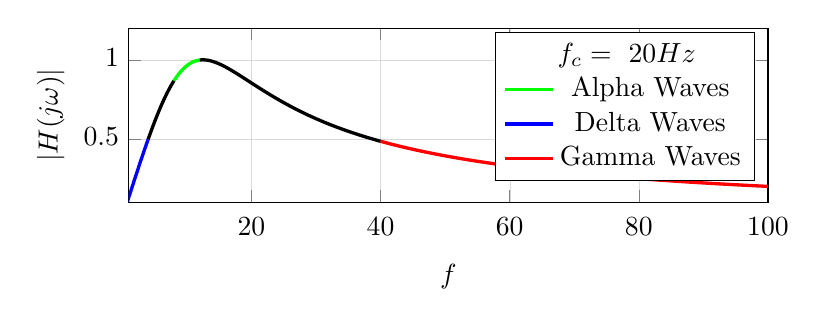
\begin{tikzpicture}[
    declare function={
      mag1(\omega)= \omega * 2 * pi * 0.020404479883576326;
      mag2(\omega)= 1 /sqrt((1 - (\omega * 2 * pi)^2 * 0.00016237369173451567)^2 + (\omega * 2 * pi * 0.020404479883576326)^2);
      mag(\omega) = mag1(\omega) * mag2(\omega);
      alpha(\omega) = mag(\omega) * (\omega >=8) * (\omega <= 12);
      delta(\omega) = mag(\omega) * (\omega <= 4);
      gamma(\omega) = mag(\omega) * (\omega > 40);
      mid1(\omega) = mag(\omega) * (\omega >= 4) * (\omega <= 8);
      mid2(\omega) = mag(\omega) * (\omega >= 12) * (\omega <= 40);
      % Straight line bode approximation
      % mag(\omega)= (\omega < 10^8) * (1) +
      %           (\omega >= 10^8) * (10^8 / \omega)
    }
  ]
  \begin{axis}[
    typeset ticklabels with strut,
    ymin=0.1, ymax=1.2, ylabel=$|H(j \omega)|$,
    xmin=1, xmax=100, xlabel=$f$,
    % xticklabels={$0.02$,$0.2$,$2$,$20$,$200$, $2000$, $20000$},
    domain=1:1000,
    grid=both, grid style={line width=.1pt, draw=gray!30},
    width=\textwidth * 0.8,
    height=\textwidth / 3.2,
  ]
    \addlegendimage{empty legend};
    \addlegendentry{\hspace{-.6cm}$f_{c} = \ 20 Hz$};
    \addplot [domain=8.001:11.999,green,very thick,samples = 200] {alpha(x)};
    \addlegendentry{Alpha Waves}
    \addplot [domain=0.5:3.999, blue,very thick,samples = 200] {delta(x)};
    \addlegendentry{Delta Waves}
    \addplot [domain=40.001:100,red,very thick,samples = 200] {gamma(x)};
    \addlegendentry{Gamma Waves}
    \addplot [domain=4.001:7.999, black,very thick,samples = 200] {mid1(x)};
    \addplot [domain=12.001:39.999,black,very thick,samples = 200] {mid2(x)};
    % \addlegendentry{Delta Waves}
    % \addplot[mark=*, red] coordinates {(4,0.478)};
    % \addplot[mark=*, green] coordinates {(40,0.37)};
    % \addlegendentry{Gamma Waves}
    % \addplot[mark=*, green] coordinates {(100,0.15)};


    \end{axis}
  \end{tikzpicture}
  \end{figure}
  }
  \qitem We again notice that while the filter is attenuating the necessary frequencies, it isn't doing that good of a job. Try plotting the responses if we had multiple filters cascaded with buffers similar to part (g).

  \ws{
  \vspace{200px}
  }

  \sol {
  We again first plot the response with one buffer.
  Notice however, that if we increase the number of buffers, while we attenuate the Delta and Gamma waves, since we are taking the gain to the $n^{th}$ power, we lose a significant amount of gain. Therefore, a tradeoff of attenuating the noise vs getting a stronger gain must be made.

  \begin{figure}[h]
  \centering

  \textbf{Magnitude Plot (One Buffer):}

  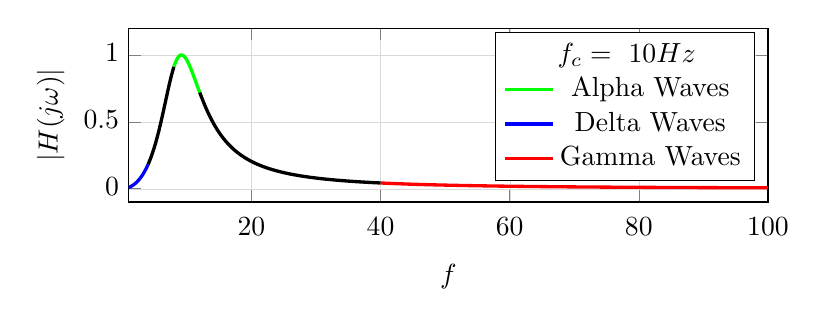
\begin{tikzpicture}[
    declare function={
      mag1(\omega)= \omega * 2 * pi * 0.015157613627799554;
      mag2(\omega)= 1 /sqrt((1 - (\omega * 2 * pi)^2 * 0.00030155114179267195)^2 + (\omega * 2 * pi * 0.015157613627799554)^2);
      mag(\omega) = (mag1(\omega) * mag2(\omega))^2;
      alpha(\omega) = mag(\omega) * (\omega >=8) * (\omega <= 12);
      delta(\omega) = mag(\omega) * (\omega <= 4);
      gamma(\omega) = mag(\omega) * (\omega > 40);
      mid1(\omega) = mag(\omega) * (\omega >= 4) * (\omega <= 8);
      mid2(\omega) = mag(\omega) * (\omega >= 12) * (\omega <= 40);
      % Straight line bode approximation
      % mag(\omega)= (\omega < 10^8) * (1) +
      %           (\omega >= 10^8) * (10^8 / \omega)
    }
  ]
  \begin{axis}[
    typeset ticklabels with strut,
    ymin=-0.1, ymax=1.2, ylabel=$|H(j \omega)|$,
    xmin=1, xmax=100, xlabel=$f$,
    % xticklabels={$0.02$,$0.2$,$2$,$20$,$200$, $2000$, $20000$},
    domain=1:1000,
    grid=both, grid style={line width=.1pt, draw=gray!30},
    width=\textwidth * 0.8,
    height=\textwidth / 3.2,
  ]
    \addlegendimage{empty legend};
    \addlegendentry{\hspace{-.6cm}$f_{c} = \ 10 Hz$};
    \addplot [domain=8.001:11.999,green,very thick,samples = 200] {alpha(x)};
    \addlegendentry{Alpha Waves}
    \addplot [domain=0.5:3.999, blue,very thick,samples = 200] {delta(x)};
    \addlegendentry{Delta Waves}
    \addplot [domain=40.001:100,red,very thick,samples = 200] {gamma(x)};
    \addlegendentry{Gamma Waves}
    \addplot [domain=4.001:7.999, black,very thick,samples = 200] {mid1(x)};
    \addplot [domain=12.001:39.999,black,very thick,samples = 200] {mid2(x)};
    % \addlegendentry{Delta Waves}
    % \addplot[mark=*, red] coordinates {(4,0.478)};
    % \addplot[mark=*, green] coordinates {(40,0.37)};
    % \addlegendentry{Gamma Waves}
    % \addplot[mark=*, green] coordinates {(100,0.15)};


    \end{axis}
  \end{tikzpicture}
  \end{figure}

\begin{figure}[h]
  \centering

  \textbf{Magnitude Plot (Five Buffers):}

  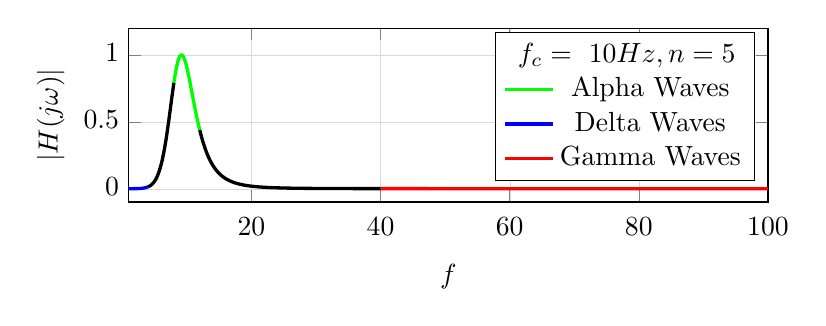
\begin{tikzpicture}[
    declare function={
      mag1(\omega)= \omega * 2 * pi * 0.015157613627799554;
      mag2(\omega)= 1 /sqrt((1 - (\omega * 2 * pi)^2 * 0.00030155114179267195)^2 + (\omega * 2 * pi * 0.015157613627799554)^2);
      mag(\omega) = (mag1(\omega) * mag2(\omega))^5;
      alpha(\omega) = mag(\omega) * (\omega >=8) * (\omega <= 12);
      delta(\omega) = mag(\omega) * (\omega <= 4);
      gamma(\omega) = mag(\omega) * (\omega > 40);
      mid1(\omega) = mag(\omega) * (\omega >= 4) * (\omega <= 8);
      mid2(\omega) = mag(\omega) * (\omega >= 12) * (\omega <= 40);
      % Straight line bode approximation
      % mag(\omega)= (\omega < 10^8) * (1) +
      %           (\omega >= 10^8) * (10^8 / \omega)
    }
  ]
  \begin{axis}[
    typeset ticklabels with strut,
    ymin=-0.1, ymax=1.2, ylabel=$|H(j \omega)|$,
    xmin=1, xmax=100, xlabel=$f$,
    % xticklabels={$0.02$,$0.2$,$2$,$20$,$200$, $2000$, $20000$},
    domain=1:1000,
    grid=both, grid style={line width=.1pt, draw=gray!30},
    width=\textwidth * 0.8,
    height=\textwidth / 3.2,
  ]
    \addlegendimage{empty legend};
    \addlegendentry{\hspace{-.6cm}$f_{c} = \ 10 Hz, n = 5$};
    \addplot [domain=8.001:11.999,green,very thick,samples = 200] {alpha(x)};
    \addlegendentry{Alpha Waves}
    \addplot [domain=0.5:3.999, blue,very thick,samples = 200] {delta(x)};
    \addlegendentry{Delta Waves}
    \addplot [domain=40.001:100,red,very thick,samples = 200] {gamma(x)};
    \addlegendentry{Gamma Waves}
    \addplot [domain=4.001:7.999, black,very thick,samples = 200] {mid1(x)};
    \addplot [domain=12.001:39.999,black,very thick,samples = 200] {mid2(x)};
    % \addlegendentry{Delta Waves}
    % \addplot[mark=*, red] coordinates {(4,0.478)};
    % \addplot[mark=*, green] coordinates {(40,0.37)};
    % \addlegendentry{Gamma Waves}
    % \addplot[mark=*, green] coordinates {(100,0.15)};


    \end{axis}
  \end{tikzpicture}
  \end{figure}

\begin{figure}[h]
  \centering

  \textbf{Magnitude Plot (Ten Buffers):}

  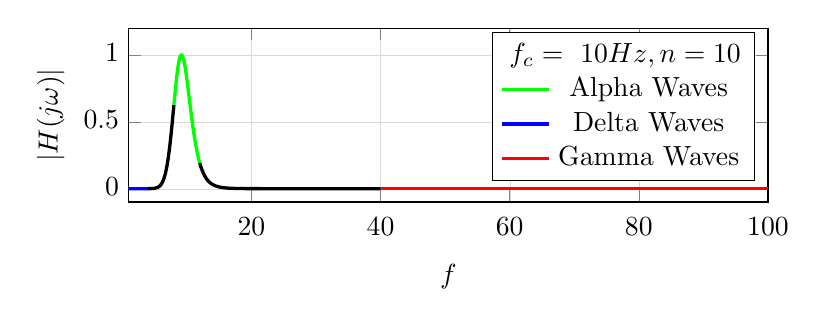
\begin{tikzpicture}[
    declare function={
      mag1(\omega)= \omega * 2 * pi * 0.015157613627799554;
      mag2(\omega)= 1 /sqrt((1 - (\omega * 2 * pi)^2 * 0.00030155114179267195)^2 + (\omega * 2 * pi * 0.015157613627799554)^2);
      mag(\omega) = (mag1(\omega) * mag2(\omega))^10;
      alpha(\omega) = mag(\omega) * (\omega >=8) * (\omega <= 12);
      delta(\omega) = mag(\omega) * (\omega <= 4);
      gamma(\omega) = mag(\omega) * (\omega > 40);
      mid1(\omega) = mag(\omega) * (\omega >= 4) * (\omega <= 8);
      mid2(\omega) = mag(\omega) * (\omega >= 12) * (\omega <= 40);
      % Straight line bode approximation
      % mag(\omega)= (\omega < 10^8) * (1) +
      %           (\omega >= 10^8) * (10^8 / \omega)
    }
  ]
  \begin{axis}[
    typeset ticklabels with strut,
    ymin=-0.1, ymax=1.2, ylabel=$|H(j \omega)|$,
    xmin=1, xmax=100, xlabel=$f$,
    % xticklabels={$0.02$,$0.2$,$2$,$20$,$200$, $2000$, $20000$},
    domain=1:1000,
    grid=both, grid style={line width=.1pt, draw=gray!30},
    width=\textwidth * 0.8,
    height=\textwidth / 3.2,
  ]
    \addlegendimage{empty legend};
    \addlegendentry{\hspace{-.6cm}$f_{c} = \ 10 Hz, n = 10$};
    \addplot [domain=8.001:11.999,green,very thick,samples = 200] {alpha(x)};
    \addlegendentry{Alpha Waves}
    \addplot [domain=0.5:3.999, blue,very thick,samples = 200] {delta(x)};
    \addlegendentry{Delta Waves}
    \addplot [domain=40.001:100,red,very thick,samples = 200] {gamma(x)};
    \addlegendentry{Gamma Waves}
    \addplot [domain=4.001:7.999, black,very thick,samples = 200] {mid1(x)};
    \addplot [domain=12.001:39.999,black,very thick,samples = 200] {mid2(x)};
    % \addlegendentry{Delta Waves}
    % \addplot[mark=*, red] coordinates {(4,0.478)};
    % \addplot[mark=*, green] coordinates {(40,0.37)};
    % \addlegendentry{Gamma Waves}
    % \addplot[mark=*, green] coordinates {(100,0.15)};


    \end{axis}
  \end{tikzpicture}
  \end{figure}

  \begin{figure}[h]
  \centering

  \textbf{Magnitude Plot (One Buffer):}

  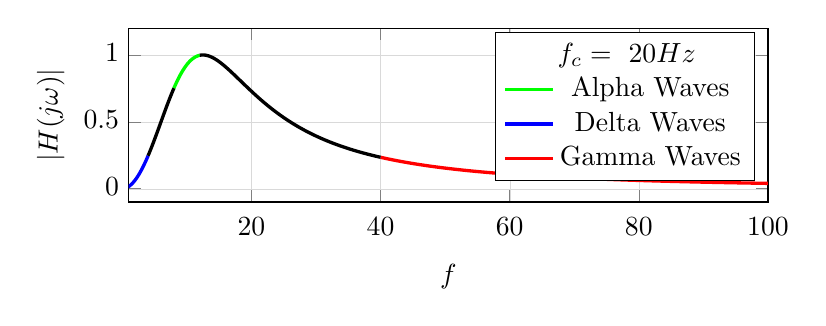
\begin{tikzpicture}[
    declare function={
      mag1(\omega)= \omega * 2 * pi * 0.020404479883576326;
      mag2(\omega)= 1 /sqrt((1 - (\omega * 2 * pi)^2 * 0.00016237369173451567)^2 + (\omega * 2 * pi * 0.020404479883576326)^2);
      mag(\omega) = (mag1(\omega) * mag2(\omega))^2;
      alpha(\omega) = mag(\omega) * (\omega >=8) * (\omega <= 12);
      delta(\omega) = mag(\omega) * (\omega <= 4);
      gamma(\omega) = mag(\omega) * (\omega > 40);
      mid1(\omega) = mag(\omega) * (\omega >= 4) * (\omega <= 8);
      mid2(\omega) = mag(\omega) * (\omega >= 12) * (\omega <= 40);
      % Straight line bode approximation
      % mag(\omega)= (\omega < 10^8) * (1) +
      %           (\omega >= 10^8) * (10^8 / \omega)
    }
  ]
  \begin{axis}[
    typeset ticklabels with strut,
    ymin=-0.1, ymax=1.2, ylabel=$|H(j \omega)|$,
    xmin=1, xmax=100, xlabel=$f$,
    % xticklabels={$0.02$,$0.2$,$2$,$20$,$200$, $2000$, $20000$},
    domain=1:1000,
    grid=both, grid style={line width=.1pt, draw=gray!30},
    width=\textwidth * 0.8,
    height=\textwidth / 3.2,
  ]
    \addlegendimage{empty legend};
    \addlegendentry{\hspace{-.6cm}$f_{c} = \ 20 Hz$};
    \addplot [domain=8.001:11.999,green,very thick,samples = 200] {alpha(x)};
    \addlegendentry{Alpha Waves}
    \addplot [domain=0.5:3.999, blue,very thick,samples = 200] {delta(x)};
    \addlegendentry{Delta Waves}
    \addplot [domain=40.001:100,red,very thick,samples = 200] {gamma(x)};
    \addlegendentry{Gamma Waves}
    \addplot [domain=4.001:7.999, black,very thick,samples = 200] {mid1(x)};
    \addplot [domain=12.001:39.999,black,very thick,samples = 200] {mid2(x)};
    % \addlegendentry{Delta Waves}
    % \addplot[mark=*, red] coordinates {(4,0.478)};
    % \addplot[mark=*, green] coordinates {(40,0.37)};
    % \addlegendentry{Gamma Waves}
    % \addplot[mark=*, green] coordinates {(100,0.15)}
    \end{axis}
  \end{tikzpicture}
  \end{figure}

  \begin{figure}[h]
  \centering

  \textbf{Magnitude Plot (Five Buffers):}

  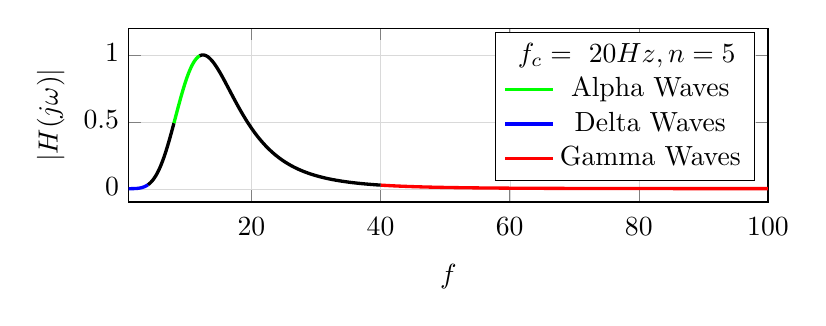
\begin{tikzpicture}[
    declare function={
      mag1(\omega)= \omega * 2 * pi * 0.020404479883576326;
      mag2(\omega)= 1 /sqrt((1 - (\omega * 2 * pi)^2 * 0.00016237369173451567)^2 + (\omega * 2 * pi * 0.020404479883576326)^2);
      mag(\omega) = (mag1(\omega) * mag2(\omega))^5;
      alpha(\omega) = mag(\omega) * (\omega >=8) * (\omega <= 12);
      delta(\omega) = mag(\omega) * (\omega <= 4);
      gamma(\omega) = mag(\omega) * (\omega > 40);
      mid1(\omega) = mag(\omega) * (\omega >= 4) * (\omega <= 8);
      mid2(\omega) = mag(\omega) * (\omega >= 12) * (\omega <= 40);
      % Straight line bode approximation
      % mag(\omega)= (\omega < 10^8) * (1) +
      %           (\omega >= 10^8) * (10^8 / \omega)
    }
  ]
  \begin{axis}[
    typeset ticklabels with strut,
    ymin=-0.1, ymax=1.2, ylabel=$|H(j \omega)|$,
    xmin=1, xmax=100, xlabel=$f$,
    % xticklabels={$0.02$,$0.2$,$2$,$20$,$200$, $2000$, $20000$},
    domain=1:1000,
    grid=both, grid style={line width=.1pt, draw=gray!30},
    width=\textwidth * 0.8,
    height=\textwidth / 3.2,
  ]
    \addlegendimage{empty legend};
    \addlegendentry{\hspace{-.6cm}$f_{c} = \ 20 Hz, n = 5$};
    \addplot [domain=8.001:11.999,green,very thick,samples = 200] {alpha(x)};
    \addlegendentry{Alpha Waves}
    \addplot [domain=0.5:3.999, blue,very thick,samples = 200] {delta(x)};
    \addlegendentry{Delta Waves}
    \addplot [domain=40.001:100,red,very thick,samples = 200] {gamma(x)};
    \addlegendentry{Gamma Waves}
    \addplot [domain=4.001:7.999, black,very thick,samples = 200] {mid1(x)};
    \addplot [domain=12.001:39.999,black,very thick,samples = 200] {mid2(x)};
    % \addlegendentry{Delta Waves}
    % \addplot[mark=*, red] coordinates {(4,0.478)};
    % \addplot[mark=*, green] coordinates {(40,0.37)};
    % \addlegendentry{Gamma Waves}
    % \addplot[mark=*, green] coordinates {(100,0.15)}
    \end{axis}
  \end{tikzpicture}
  \end{figure}

  \begin{figure}[h]
  \centering

  \textbf{Magnitude Plot (Ten Buffers):}

  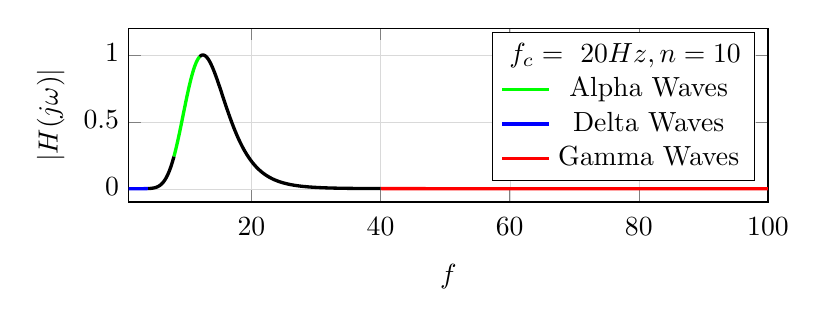
\begin{tikzpicture}[
    declare function={
      mag1(\omega)= \omega * 2 * pi * 0.020404479883576326;
      mag2(\omega)= 1 /sqrt((1 - (\omega * 2 * pi)^2 * 0.00016237369173451567)^2 + (\omega * 2 * pi * 0.020404479883576326)^2);
      mag(\omega) = (mag1(\omega) * mag2(\omega))^10;
      alpha(\omega) = mag(\omega) * (\omega >=8) * (\omega <= 12);
      delta(\omega) = mag(\omega) * (\omega <= 4);
      gamma(\omega) = mag(\omega) * (\omega > 40);
      mid1(\omega) = mag(\omega) * (\omega >= 4) * (\omega <= 8);
      mid2(\omega) = mag(\omega) * (\omega >= 12) * (\omega <= 40);
      % Straight line bode approximation
      % mag(\omega)= (\omega < 10^8) * (1) +
      %           (\omega >= 10^8) * (10^8 / \omega)
    }
  ]
  \begin{axis}[
    typeset ticklabels with strut,
    ymin=-0.1, ymax=1.2, ylabel=$|H(j \omega)|$,
    xmin=1, xmax=100, xlabel=$f$,
    % xticklabels={$0.02$,$0.2$,$2$,$20$,$200$, $2000$, $20000$},
    domain=1:1000,
    grid=both, grid style={line width=.1pt, draw=gray!30},
    width=\textwidth * 0.8,
    height=\textwidth / 3.2,
  ]
    \addlegendimage{empty legend};
    \addlegendentry{\hspace{-.6cm}$f_{c} = \ 20 Hz, n = 10$};
    \addplot [domain=8.001:11.999,green,very thick,samples = 200] {alpha(x)};
    \addlegendentry{Alpha Waves}
    \addplot [domain=0.5:3.999, blue,very thick,samples = 200] {delta(x)};
    \addlegendentry{Delta Waves}
    \addplot [domain=40.001:100,red,very thick,samples = 200] {gamma(x)};
    \addlegendentry{Gamma Waves}
    \addplot [domain=4.001:7.999, black,very thick,samples = 200] {mid1(x)};
    \addplot [domain=12.001:39.999,black,very thick,samples = 200] {mid2(x)};
    % \addlegendentry{Delta Waves}
    % \addplot[mark=*, red] coordinates {(4,0.478)};
    % \addplot[mark=*, green] coordinates {(40,0.37)};
    % \addlegendentry{Gamma Waves}
    % \addplot[mark=*, green] coordinates {(100,0.15)}
    \end{axis}
  \end{tikzpicture}
  \end{figure}

  % \begin{figure}[!ht]
  % \centering
  % \begin{tikzpicture}[
  %   declare function={
  %     phase(\omega)= -rad(atan((\omega * 2 * pi * 0.0189)/((1 - (\omega * 2 * pi)^2 * 0.0002010341)));
  %     % Straight line bode approximation
  %     % mag(\omega)= (\omega < 10^8) * (1) +
  %     %           (\omega >= 10^8) * (10^8 / \omega)
  %   }
  % ]
  % \begin{axis}[
  %   typeset ticklabels with strut,
  %   ymin= 0.3, ymax=-3.5, ylabel=$\angle H(j \omega)$, ytick={-2*pi, -3*pi/2, -pi, -pi/2, 0},
  %   yticklabels={$0$,$-\frac{\pi}{2}$,$-\pi$,$-\frac{3 \pi}{2}$,$\frac{3\pi}{2}$},
  %   xmin=1, xmax=100, xlabel=$f$,
  %   % xticklabels={$0.02$,$0.2$,$2$,$20$,$200$, $2000$, $20000$},
  %   domain=1:1000,
  %   grid=both, grid style={line width=.1pt, draw=gray!30},
  %   width=\textwidth * 0.8,
  %   height=\textwidth / 3.2,
  %   samples = 900
  % ]
  %   \addplot [blue,very thick] {phase(x)};
  %   \end{axis}
  % \end{tikzpicture}
  % \end{figure}
  }

\end{enumerate}
